\documentclass{article}

\usepackage{booktabs}
\usepackage{tabularx}

\title{Title of Project}

\author{Team Name
		\\ Taylor de Vet
    \\ Glenne Grossman
		\\ Jamal Habash
		\\ Cameron Nowikow
}

\date{November 6th, 2017}



\begin{document}

\newpage

\maketitle

<<<<<<< HEAD
\newpage
=======
We write introduction stuff here

\section{Introduction}

Information is a vital resource, espcially in the context of Healthcare. When a patient's health is at risk, their medical history becomes the most important piece of information in providing them with appropriate care.

At present, in Ontario, there exists no secure, liftime record of your health history. When faced with a problem, healthcare providers are left without the big picture, and often fumble for generic solutions, instead of catering care to each individual.

One situation where this information gap is the most noticiable is when patients recieve care from Emergency First Responders (EFRs). Today, EFRs respond to emergencies knowing little or nothing about the people in their care. This is unforunate, considering how beneficial information is in improving patient outcomes. \iffalse For example, nursing homes often carry documents that contain health information on their residents. This information, including medications, allergies and diagonsed disorders gives EFRs an important base-knowledge for how assessing a patient. \fi

The objective of this capstone is to therefore develop an information management system that stores health records for access by patients, and their healthcare providers. Specifically, the goal of the capstone is to develop software that can be used by Emergency First Responders to access patient health records while responding to a call. This will provide EFRs with information vital to providing patients with the best care possible. In addition to software, hardware will be developed that provides EFRs with a means to quickly identify patients and access there information on the system. This hardware will also include a real-time vitals tracker, which has the potential to track vitals (i.e. Heart Rate) deemed useful by EFRs.


\section{Resources}
The following is a list of resources that have been used in the research process thus far.
\begin{itemize}
\item Currently we are in communication with 2 Ontario Paramedics who have provided us insight on the various issues and difficulties that they run into on a daily basis.
\item We are also in communication with Dr. Aleksandar Jeremic and Dr. Hubert deBruin to gather their insight on this project.
\item We have access to a Bioinstrumentation laboratory at McMaster University which will allow us to test our hardware components both on patients and patient simulators to ensure everything is working properly and safely.
\end{itemize}



\section{Description}

\subsection{Motivation}
Cam
\subsection{Background}
All of us
\subsection{Project details milestone and completion}
Glenne
\section{Scheduling}
Glenne
\section{Assumptions and Risks}

\subsection{Assumptions}

As of present, it is assumed that there is no centralized health record that contains the cumulative health information of Ontario residents. The information required for this system is not available today, and we are developing software based on the assumption, that in the future, this information will need to be collected.

For this capstone, the software being built is focused on how health information is to be handeled, and the best way to present this information to the user, specifically EFRs. As a component of the capstone, we will brainstorm the best methods by which to collect and aggregate health records, however the means by which to collect these records will not be built.

\subsection{Risks}

Software development is inherently difficult to estimate and schedule. While we have done our best to estimate the time required to reach our goals, we do not have experience with large-scale software projects. Without experience, we do not truly know the length of time each component of the system will take to develop, and there is a risk we may not meet our inital development goals. To mitigate this risk, we will be having weekly meetings to gauge our progress, allowing us to modify our goals as required. Additonally, we have been conservative in our deliverable estimates, giving us ample opporunity to add, or remove features to the software depending on the availability of time.

\iffalse
have been conservative in our deliverable estimates, and will be having weekly meetings in order to guage the progress of development as we go along. This will allow us to remove, or add features to the software depending on the availability of time.




------------------

Random stuff :P ignore:

As of now, there is no centralized health record that contains the cumulative health information of Ontario residents.

We are developing software based on the assumption, that in the future, this information will need to be collected, and we will brainstorm the best methods by which to aggregate this information. The software being built is focused on how to handle the information and present the information, vs how the information is inputed into the system

It is assuming that we are not focused on how to input the information, so much as how to handle and present the information to the correct user.

It is assumed that the information required for this system is not available today

\fi

\section{Deliverables}
\subsection{Bronze}
The bronze category is the bare minimum of what is to be accomplished for the final product. The following are Bronze Level goals.
\begin{itemize}
  \item Working User Interface
	\begin{itemize}
	\item The user interface for this applivation is the most important aspect as this is what the Paramedic or Emergency personel will be looking at when inputting and acessing data. At this level, the user interface must have the following functionality. Firstly
	\item Firstly, the application must be compatible with iOS and Android devices. There is currently no standardization for the tools that Paramedics use and having an app that can be used on any platform makes it more readily useable with current technology.
	\item Secondly, this application must be able to access a database of health information assumed to exist and display said data on the screen of the users device. This will be done in a layout similar to the software
	\end{itemize}
  \item Another entry in the list
\end{itemize}
Taylor

\section{Conclusion}

Throughout the development process, both the software and hardware will be tested to ensure it meets design requirements. In terms of software, each module will be verified using test cases that have known outcomes to ensure functionality. The hardware will be tested in a similar way, using test cases to verify the hardware meets specification.

An example of real-world testing that can be used is in verifying the pulse-sensing capabilites. The hardware can be tested on a group member with a known pulse (through traditional human pulse reading), to ensure that the device senses pulses correctly.

\section{Summary}


>>>>>>> 908ed5e1f637e1e15d98ed30be42968e8e844e47


\section{Introduction}

Information is a vital resource, especially in the context of Healthcare. When a patient's health is at risk, their medical history becomes the most important piece of information in providing them with appropriate care \cite{web1}.

At present, there exists no secure, lifetime record of your health history \cite{Street2014}. When faced with a problem, healthcare providers are left without the big picture, and often fumble for generic solutions, instead of catering care to each individual. In Ontario, the government is addressing this problem through a new initiative called eHealth Ontario; a group focused on researching how to best connect patients and providers through digital technology and information \cite{web1}. The initiative has developed a framework for building the future of ``interoperable electronic health records (EHR) for Ontarians'', which outlines and defines how a comprehensive EHR may be developed \cite{b1}.

Among technical details, the blueprint defines how ``information access portals'' may be used to distribute and present information to stakeholders, ensuring patients and providers are presented with the information most relevant to them. The blueprint further identifies key areas that may require unique access portals, such as hospitals, community care facilities and pharmacies \cite{Street2014}.

One stakeholder identified as requiring an information access portal are Emergency First Responders (EFRs). Today, EFRs respond to emergencies knowing little or nothing about the people in their care. This results in a noticeable information gap that reduces the effectiveness of EFRs, and the negatively impacts the outcomes of their patients. \iffalse reducing the effectiveness of EFRs, and   during treatment. This is unfortunate, considering how beneficial information is in improving patient outcomes. \fi

\iffalse The objective of this capstone is to therefore develop an information management system that stores health records for access by patients, and their healthcare providers. \fi The objective of this capstone is to therefore develop ``information access portal'' (IAP) software, that can be used by EFRs to obtain and create patient health records while responding to a call. In addition to software, hardware will be developed to provide EFRs with a means to track and store a patients vitals (i.e. Heart Rate) in real-time. Such information can be useful in determining the status of a patient, and in the case of a large-scale event, allow responders to allocate their resources and time to the people that need it most. Vitals information can be stored and displayed through the information access portal, functioning as a proof-of-concept for a more comprehensive emergency response event tracking system in the future. The ideal system would then consist of an information access portal that allows responders to not only access medical information, but work in conjunction with hardware to create a record of the emergency for use by other medical professionals.


\section{Background}

\subsection{eHealth Ontario}

Throughout Ontario, there is a clear desire to bring healthcare into the digital age by using software to improve access to medical information. The province intends to use a service-oriented architecture to allow for the development of components (i.e. IAPs) that distribute information between systems using a standard protocol known as the Health Information Access Layer (HIAL). HIAL will act as ``the broker and mediator for information exchange, ensuring that all [software] abide[s] by a common set of rules'' \cite{b1}. The intention of the government is to have a comprehensive and secure electronic health record, that may be accessed by HIAL-supporting software. This software (i.e. IAPs) may be developed by any vendor to support any patient or healthcare professional as the vendor sees fit. A systems diagram of Ontario's future eHealth infrastructure can be seen in figure~\ref{fig:eHealth1} below.

\begin{figure}[h]
  \centering
  \includegraphics[width=\linewidth]{diagramOntario.png}
  \captionsetup{format=hang}
  \caption[Ontario eHealth Systems View]{A systems view of Ontario's planned eHealth infrastructure, showing ``how EHR resources and services [will be] integrated and deployed.'' \cite{b1}}
  \label{fig:eHealth1}
\end{figure}

\subsection{Talking with Paramedics}

In regards to software and hardware for EFRs, we talked to a number of paramedics about how technology can support and improve the care they provide. Currently, EFRs use software such as the system seen in figure~\ref{fig:iMed1} on page~\pageref{fig:iMed1}, to guide them through collecting data that may be important to a patients health. These systems are cumbersome, require time to fill, and are only as helpful as the information the paramedics manage to collect. Throughout our discussions, there was overwhelmingly interest in a system that could provide paramedics with patient medical history. \iffalse We discovered that any information provided to a paramedic is helpful, and can greatly improve the quality and speed of care. In general,\fi Our findings can be summarized with the following quote from paramedic Matt Sartor:

\blockquote{Nursing homes carry [transfer documents] that contain updated information on [a patient] such as: medications, allergies and diagnosed disorders; including say if they [have] had a stroke, or have dementia, and what level of cognition or communication is normal for them. This kind of information gives us as paramedics a tipping point for how we assess our patients, or how we expect to communicate with them or have them do the same with us. [This information] would be very helpful for anyone we meet. Even if it's only [medication] history and allergies, we can decipher a lot from that. Even recent visits to hospital gives us a pattern of problems with a patient.

Currently the hospital can scan their card and get all prior hospital visits and diagnoses on discharges, but it's not available or compact enough for [paramedics] to get. If somehow our laptop forms, which we have to manually input all information we can attain, could get the aforementioned information, it would largely influence our practice.
}

Matt went on to explain how there are several different documenting systems used by Paramedics in Ontario, and that none are standardized. A standard system, like the one we are developing, would improve the ability of professionals to work together, and provide patients with care.

\begin{figure}[h]
  \centering
  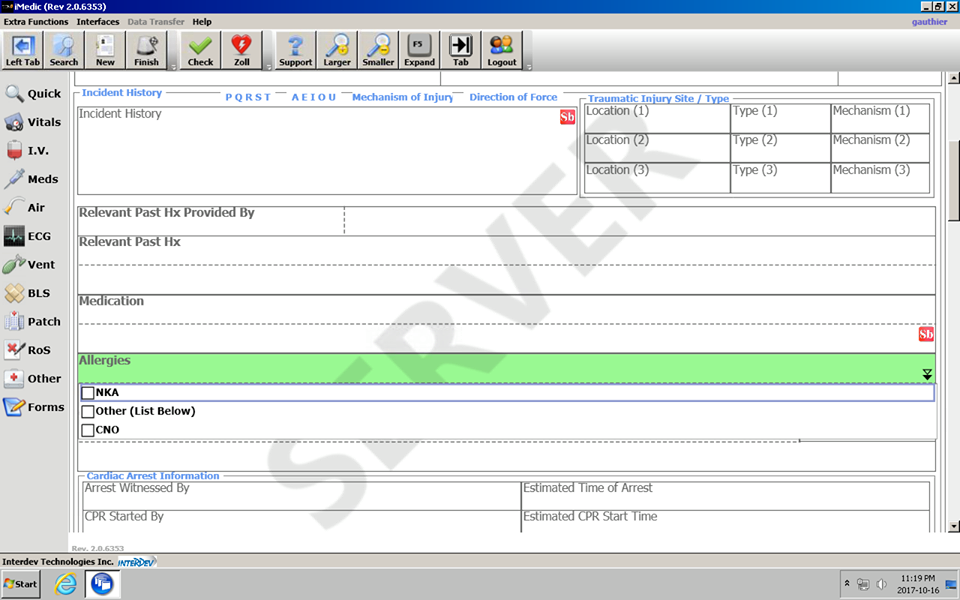
\includegraphics[width=\linewidth]{iMedic.png}
  \captionsetup{format=hang}
  \caption[Screenshot of iMedic Software]{A screenshot of the current software, iMedic, used by paramedics when responding to a call.}
  \label{fig:iMed1}
\end{figure}

As discussed, there currently exists no cumulative EHR in Ontario, and we are developing software based on the assumption that in the future an EHR will exist. The software we develop will be focused on handling, storing and presenting medical information, rather than how it will be acquired.

\subsection{Alternative Electronic Health Records}

In 2003 the World Health Organization (WHO) released a document outlining the possibility of implementing a medical information system using “smart cards”. They described how information stored on a card could be carried by patients, that when scanned, would allow professionals to see the patients medical history \cite{smartcard1}. This method of information retrieval has the medical history being stored on the card itself, which is incompatible with Ontario's future EHR infrastructure. Instead of storing medical information, we will be using health cards to identify patients and provide authentication to access a particular medical record.


\section{Software Design Component}

The software system we are designing will function as a portal to Electronic Health Records in Ontario. The main user of the system will be paramedics. In the future, we hope users will extend to all levels of the medical profession as well as the general public.
We will design an application targeted at paramedics that works on both iOS and Android phones.This application will allow paramedics to view patient information that they do not normally have access too. The app will have a loading screen, a login page, a home page, patient pages accessed by scanning health cards or inputting the health card number.


\subsection{Technology}
In order to create the Android and iOS app we will require certain technologies.
Firstly, the app will be written using React Native a javascript framework that allows apps to be written for Android and iOS concurrently. The app will require a database to store the patient information. For this, we will use Node.js however, we are assuming that in the future if our app is put to use we will easily adapt to how the EHR are stored by Ontario.


\subsection{Functional Design}
The app will have basic functional requirements as well as features we would like to implement once the basic requirements are completed.
The basic functional requirements are that the device follows the standards outlined on the ehealth blueprint documents put out by eHealth Ontario.
This document guides us through the appropriate exchange and access of information within the app.
Functionally, it will need to have a secure log-in screen for paramedics. A home screen with buttons leading to history, settings, option to connect to WiFi hardware device, and the health card scanner.
Once a hardware device or a health card are connected it will then need to bring up a patient page and show the sensor data and/or the patients EHR. The history screen for the basic requirements will simply show what patients the paramedic has treated but will not allow the paramedic more access to their information once the paramedic has closed the patient's EHR.
In future versions the paramedic will be able to record information about the particular visit into the EHR, and will be able to view these additions on the history screen. In the future additions, the sensed data will also be stored and be visible in the EHR so medical personell at a hospital or later at a doctor's visit will be able to view the patients vitals at the time of the paramedics visit.


\subsection{Non-Functional Design}
The app must have secure information storage and transmission by the standards outlined in the eHealth Blueprint. The app must have a cohesive look, including size and colour scheme in order to be easy to navigate. The app must be available in english and french. The app will be made so that the average paramedic is able to use it (assuming paramedics are males and females adults with above secondary education) and will use terms that are familiar to them.
The app must be able to run on Android and iOS devices that still recieve updates from their providers. The app must not have harsh colouring or flashing lights in order to prevent harm to the paramedics.

\documentclass{article}

\usepackage{booktabs}
\usepackage{tabularx}

\title{Hardware Design Proposal}


\begin{document}

\newpage

\maketitle
\section{Hardware Design Component}

To adequately track the vitals of a patient, there are 2 hardware components required; the sensor, and the transmitter.
\subsection{Sensor}
As this is a preliminary design, only one vital will be tracked as proof of modality so the focus will be on heart rate and blood oxygen saturation. 
A simple heart rate sensor will be constructed consisting of an infrared and red wavelength emitter and receiver as well as an amplification circuit. 
The 2 LEDS are pulsed on the skin of the patient and the reflectance of both wavelengths is measured by detectors. IR and red light scatter differently 
depending on the amount of blood in the skin at that time and the detectors pick up the reflected light from both and output the corresponding current and 
voltage. This is then amplified and is sent to a microcontroller. \par

To decrease the size of the overall sensor, an ATmega microcontroller can be used with the appropriate capacitors, oscillators, and power source to avoid the 
use of a full Arduino board. This chip will receive signals in from the pulse oximetry circuit and can calculate the heart rate, blood oxygen concentration and
 will create a pulse wave to show heart activity. These signals can then be sent out through a Wi-Fi Transceiver module to the user’s mobile device. 
\subsection{Transmitter}
All modern communication devices, such as tablets and mobile phones, can connect to auxiliary devices via Bluetooth and Wi-Fi. Bluetooth communication has 
limitations on how many devices can be connected to a parent device at any given time with the ideal number being 4. \cite{apple1} As the primary use for this device
 will be for mass accidents, being limited to 4 patients per device is impractical. Wireless internet networks such as Wi-Fi are less limited and allow for 
 10 devices to be connected at a time when using a mobile hotspot source. \cite{} When a paramedic is out in the field, a mobile internet source will be provided
 from a mobile hotspot and will have the ability to have 10 devices actively communicating with it at a time. This also allows for information to be sent to 
 the hospital in real time whereas Bluetooth communication would be limited to when the patient has already reached the hospital. Because of this we have 
 chosen to connect to our sensors through Wi-Fi with the receiver being the devices own internal Wi-Fi receiver. 
To transmit the data from the pulse oximetry sensor to the mobile device, a serial Wi-Fi transceiver module will be used. With both devices connected to 
the same wireless network, data will able to be sent serially from the sensor to the host device.  


\end{document}

\section{Conclusion}

Throughout the development process, both the software and hardware will be tested to ensure it meets design requirements. In terms of software, each module will be verified using test cases that have known outcomes to ensure functionality. 

The hardware will be tested in a similar way, using test cases to verify the hardware meets specification. The pulse oximetry circuit can be tested on a group member that has had their pulse calculated with a 3rd party device i.e. FitBit. The pulse rate from the FitBit and the circuit can be compared to test if pulse if being sensed correctly. 

The ability to transfer data from the sensor to a mobile device can be tested through a simplistic mobile application that will display the information on the users screen. 



\end{document}
